\section{Introduction}
Despite the ubiquity of online search, help-seeking remains a tedious and difficult process for many. While the Web is ripe with knowledge and expert help, using it requires switching mental context, visual attention, and input focus away from the task at hand. As the RePlay study showed, these drawbacks often prevent people from searching altogether. Though bringing the search interface closer to the user's workflow and tying in relevant context seemed to help people spend less time once they decided to search, there was still an initial barrier that prevented many from searching in the first place. 
Coming up with an appropriate search query can be prohibitively difficult for novices, who may not know the correct vocabulary [dan russell]. It also switches the user's attention from the task at hand to the task of articulating their goal in a way that will match the resources they seek. How might we lower the barrier to searching and make it easier for people to find the resources they need in the moment?

When people help each other, they often use language, gestures, and context. Our research investigates how computers might do this too. The combination has allowed people of different backgrounds to communicate information and interact. Although it is a habit of humans to incorporate language, gestures, and context into assisting others, computers do not develop this knowledge unless programmed to. 

This chapter explores how multimodal interaction might make searching easier in the moment. Different types of information lend themselves better to different modalities; leveraging the strengths of multiple modalities and integrating them smoothly can be extremely effective \cite{Oviatt1999}. For example, combining speech and pointing allows people to communicate more precisely and efficiently by using deictic terms (\textit{e.g.,} ``this'', ``here'') to refer to objects and locations \cite{Bolt1980, Linder2013}. Furthermore, using multiple modalities simultaneously can improve efficiency; \textit{e.g.,} navigating tutorial videos with speech while one's hands are busy with a physical task \cite{Chang2019}. Finally, multimodal systems can also enable more natural interaction; \textit{e.g.,} letting users describe photo edits in their own words and inferring the appropriate commands \cite{Linder2013}, or activating software commands with speech rather than memorizing keyboard shortcuts \cite{Kim2019}.

\begin{figure}
\centering
  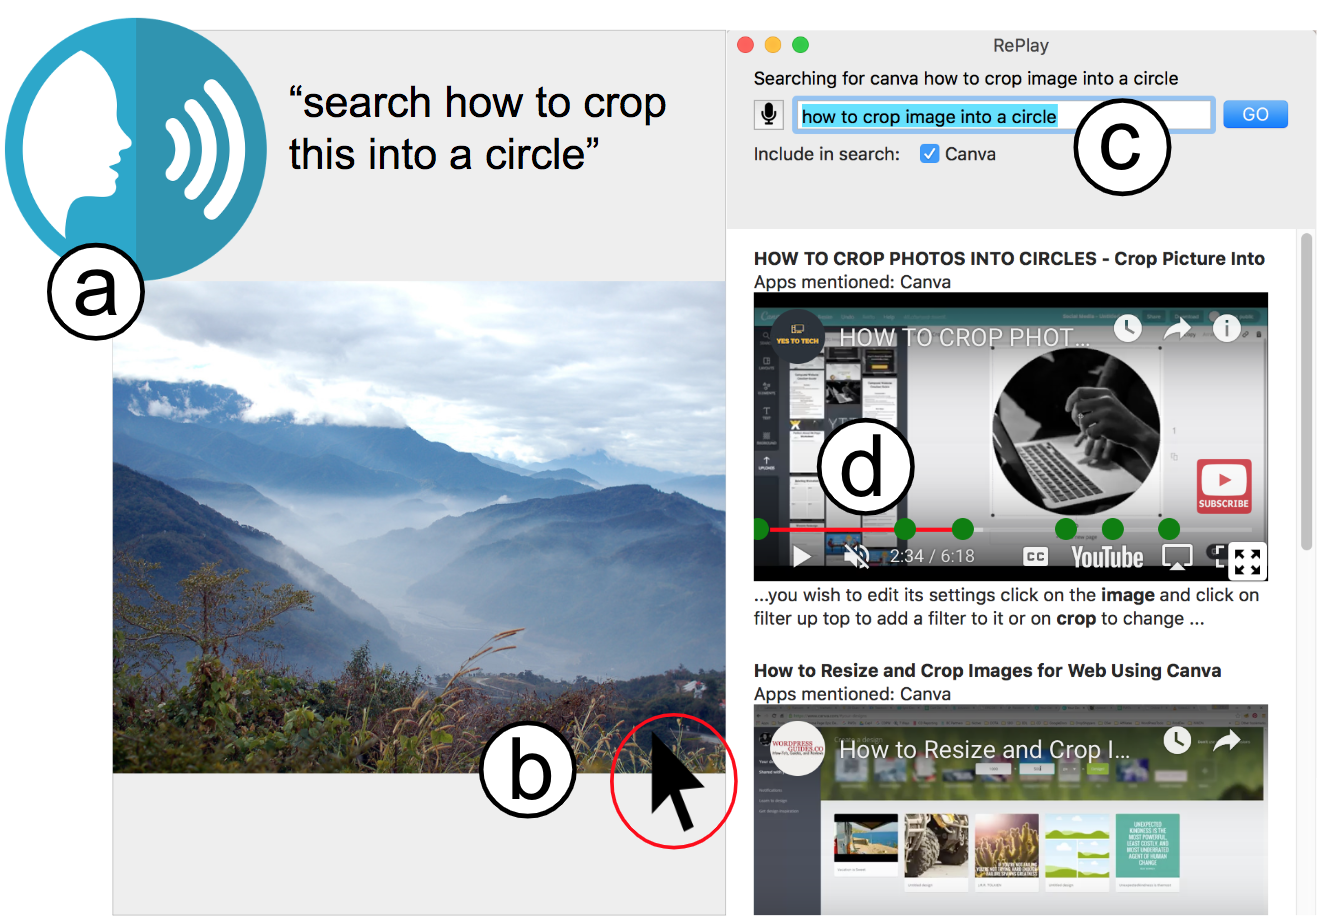
\includegraphics[width=\textwidth]{remap/figures/interface.png}
  \caption{ReMap is a multimodal search interface for finding learning videos. a) The user speaks their query. b) The user clicks on an image on the canvas while saying the word ``this.'' c) ReMap automatically changes the word ``this'' to ``image.'' d) ReMap highlights relevant moments by placing markers on the timeline of each video result.}~\label{fig:remap_interface}
  \vspace{-0.3in}
\end{figure}

We introduce ReMap, a multimodal interface for users to search for learning videos using speech and pointing, without taking their hands (or mouse) off their current task. ReMap builds on the existing video search interface RePlay \cite{Fraser2019}. ReMap's multimodal help search demonstrates three main design insights:
\begin{enumerate}
\item Users can initiate and dictate a search at anytime using speech, to avoid context-switching.
\item Users can point at elements in the software they are using to include their names in the search query, removing the need to remember app-specific terminology.
\item Users can play, pause, and navigate video results using speech, allowing them to simultaneously work on their task and follow along with a video tutorial.
\end{enumerate}

A study with 13 participants found that ReMap allows people to stay focused on their task while help-seeking. The study along with iterative prototyping and pilot testing also raised a number of important challenges with incorporating multimodal features into a help-seeking system.